%%%%%%%%%%%%%%%%%%%%%%%%%%%%%%%%%%%%%%%%%
% Beamer Presentation
% LaTeX Template
% Version 1.0 (10/11/12)
%
% This template has been downloaded from:
% http://www.LaTeXTemplates.com
%
% License:
% CC BY-NC-SA 3.0 (http://creativecommons.org/licenses/by-nc-sa/3.0/)
%
%%%%%%%%%%%%%%%%%%%%%%%%%%%%%%%%%%%%%%%%%

%----------------------------------------------------------------------------------------
%	PACKAGES AND THEMES
%----------------------------------------------------------------------------------------

\documentclass{beamer}

\mode<presentation> {

% The Beamer class comes with a number of default slide themes
% which change the colors and layouts of slides. Below this is a list
% of all the themes, uncomment each in turn to see what they look like.

%\usetheme{default}
%\usetheme{AnnArbor}
%\usetheme{Antibes}
%\usetheme{Bergen}
%\usetheme{Berkeley}
%\usetheme{Berlin}
%\usetheme{Boadilla}
%\usetheme{CambridgeUS}
%\usetheme{Copenhagen}
%\usetheme{Darmstadt}
%\usetheme{Dresden}
%\usetheme{Frankfurt}
%\usetheme{Goettingen}
%\usetheme{Hannover}
%\usetheme{Ilmenau}
%\usetheme{JuanLesPins}
%\usetheme{Luebeck}
\usetheme{Madrid}
%\usetheme{Malmoe}
%\usetheme{Marburg}
%\usetheme{Montpellier}
%\usetheme{PaloAlto}
%\usetheme{Pittsburgh}
%\usetheme{Rochester}
%\usetheme{Singapore}
%\usetheme{Szeged}
%\usetheme{Warsaw}

% As well as themes, the Beamer class has a number of color themes
% for any slide theme. Uncomment each of these in turn to see how it
% changes the colors of your current slide theme.

%\usecolortheme{albatross}
%\usecolortheme{beaver}
%\usecolortheme{beetle}
%\usecolortheme{crane}
%\usecolortheme{dolphin}
%\usecolortheme{dove}
%\usecolortheme{fly}
%\usecolortheme{lily}
%\usecolortheme{orchid}
%\usecolortheme{rose}
%\usecolortheme{seagull}
%\usecolortheme{seahorse}
\usecolortheme{whale}
%\usecolortheme{wolverine}

\setbeamertemplate{footline} % To remove the footer line in all slides uncomment this line
%\setbeamertemplate{footline}[page number] % To replace the footer line in all slides with a simple slide count uncomment this line

\setbeamertemplate{navigation symbols}{} % To remove the navigation symbols from the bottom of all slides uncomment this line

}

\usepackage{graphicx} % Allows including images
\usepackage{booktabs} % Allows the use of \toprule, \midrule and \bottomrule in tables
\usepackage{sansmathaccent}
\usepackage{amsmath}
\pdfmapfile{+sansmathaccent.map}

\usepackage{tikz}
\usetikzlibrary{trees, arrows, shapes, positioning}
%----------------------------------------------------------------------------------------
%	TITLE PAGE
%----------------------------------------------------------------------------------------

\title[Intro to Graphs]{Introduction to Graphs} % The short title appears at the bottom of every slide, the full title is only on the title page

%\author{John Smith} % Your name
\institute[BYU] % Your institution as it will appear on the bottom of every slide, may be shorthand to save space
{
Brigham Young University \\ % Your institution for the title page
\medskip
%\textit{john@smith.com} % Your email address
}
\date{\today} % Date, can be changed to a custom date

\begin{document}

\begin{frame}
\titlepage % Print the title page as the first slide
\end{frame}

%\begin{frame}
%\frametitle{Overview} % Table of contents slide, comment this block out to remove it
%\tableofcontents % Throughout your presentation, if you choose to use \section{} and %\subsection{} commands, these will automatically be printed on this slide as an overview of your presentation
%\end{frame}

%----------------------------------------------------------------------------------------
%	PRESENTATION SLIDES
%----------------------------------------------------------------------------------------

%------------------------------------------------
%\section{First Section} % Sections can be created in order to organize your presentation into %discrete blocks, all sections and subsections are automatically printed in the table of contents %as an overview of the talk
%------------------------------------------------

%\subsection{Subsection Example} % A subsection can be created just before a set of slides with %a common theme to further break down your presentation into chunks

%\begin{frame}
%\frametitle{AVL trees}
%Sed iaculis dapibus gravida. Morbi sed tortor erat, nec interdum arcu. Sed id lorem lectus. %Quisque viverra augue id sem ornare non aliquam nibh tristique. Aenean in ligula nisl. Nulla sed %tellus ipsum. Donec vestibulum ligula non lorem vulputate fermentum accumsan neque mollis.%\\~\\

%Sed diam enim, sagittis nec condimentum sit amet, ullamcorper sit amet libero. Aliquam vel dui %orci, a porta odio. Nullam id suscipit ipsum. Aenean lobortis commodo sem, ut commodo leo %gravida vitae. Pellentesque vehicula ante iaculis arcu pretium rutrum eget sit amet purus. %Integer ornare nulla quis neque ultrices lobortis. Vestibulum ultrices tincidunt libero, quis %commodo erat ullamcorper id.
%\end{frame}

%------------------------------------------------
\begin{frame}
\frametitle{Graphs}

\begin{itemize}
\item A \textbf{graph} $G  = (V,E)$ is a pair consisting of a nonempty finite set $V$ of \textbf{vertices} (nodes) and a relation $E$ on $V$ corresponding to the \textbf{edges} of the graph.
\item In other words, $E$ is a set of ordered pairs.
\item If there is a function $w: E \rightarrow \mathbb{R} $ the graph is \textbf{weighted}.
\end{itemize}
\end{frame}

%-----------------------------------------------

\begin{frame}
\frametitle{Graph Example}
\begin{center}
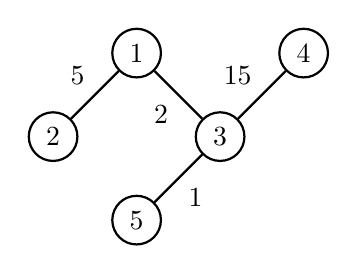
\begin{tikzpicture}[auto,node distance=1.5cm,
 thick,main node/.style={circle,draw}]
 
  \node[main node] (1) [] {1};
  \node[main node] (2) [below left of=1] {2};
  \node[main node] (3) [below right of=1] {3};
  \node[main node] (4) [above right of=3] {4};
  \node[main node] (5) [below left of=3] {5};  
  
  \foreach \s/\t/\i in {2/1/5 , 3/1/2, 3/4/15, 3/5/1 } {
   \path[draw] (\s) edge node {\i} (\t);}

\end{tikzpicture}
\end{center}
\begin{itemize}
\item $V = \{ 1,2,3,4,5\}$
\item $E = \{(1,2), (1,3), (3,4), (3,5))\}$
\item $w: (1,2) \mapsto 5, (1,3) \mapsto 2, (3,4)\mapsto 15, (3,5)\mapsto 1$
\end{itemize}

\end{frame}

%-----------------------------------------------

\begin{frame}
\frametitle{Directed Graphs}
\begin{itemize}
\item A graph is \textbf{directed} if edges only go one way.
\item When edges are not allowed to connect a node to itself, it is called \textbf{simple}.
\end{itemize}
\begin{center}
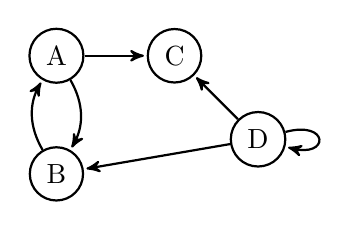
\begin{tikzpicture}[->,>=stealth',shorten >=1pt,auto,node distance=1.5cm,thick,main node/.style={circle,draw}]
  \node[main node] (A) [] {A};
  \node[main node] (B) [below of=A] {B};
  \node[main node] (C) [right of=A] {C};
  \node[main node] (D) [below right of=C] {D};
  \foreach \s/\t in {A/C, D/B, D/C} {\path[draw] (\s) edge (\t);}
  \path[]
 	(A) edge [bend left]  (B)
	(B) edge [bend left]  (A)
 	(D) edge [loop right] (D);
\end{tikzpicture}
\end{center}
\begin{itemize}
\item This graph is not simple because D connects to itself.
\item $ V = \{A,B,C,D \}$
\item $ E = \{(A,B),(A,C),(B,A),(D,B),(D,C),(D,D)\}$
\end{itemize}

\end{frame}

%----------------------------------------------
\begin{frame}
\frametitle{Definitions}
\begin{itemize}
\item The \textbf{neighborhood} $N_i \subset V$ of a vertex $v_i \in V$ is the set of nodes that are connected to $v_i$.
    \begin{itemize}
    \item $N_i = \{ v_j \in V | (v_i, v_j) \in E \}$
    \end{itemize}

\end{itemize}

\begin{columns}[c]
\column{.5\textwidth}
\begin{center}
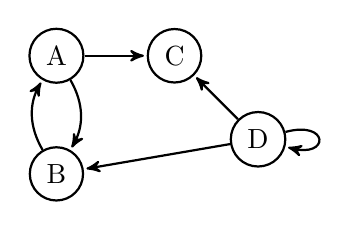
\begin{tikzpicture}[->,>=stealth',shorten >=1pt,auto,node distance=1.5cm,
 thick,main node/.style={circle,draw}]

  \node[main node] (A) [] {A};
  \node[main node] (B) [below of=A] {B};
  \node[main node] (C) [right of=A] {C};
  \node[main node] (D) [below right of=C] {D};

  \foreach \s/\t in {A/C, D/B, D/C} {
   \path[draw] (\s) edge (\t);}
    
  \path[]
 	(A) edge [bend left]  (B)
	(B) edge [bend left]  (A)
 	(D) edge [loop right] (D);

\end{tikzpicture}
\end{center}
\column{.5\textwidth}
\begin{itemize}
\item $N_A = \{B,C\}$
\item $N_B = \{A\}$
\item $N_C = \{ \}$
\item $N_D = \{C,B,D\}$
\end{itemize}
\end{columns}

\end{frame}
%-----------------------------------------------
\begin{frame}
\frametitle{Definitions}

\begin{itemize}
\item A \textbf{path} of length $m$ in $G(V,E)$ is a sequence of vertices $v_{i_1},v_{i_2},...,v_{i_m}$ where $(v_{i_k},v_{i_{k+1}}) \in E$ for all $k = 1, 2, ... , m-1$.
\item The first node in a path is the \textbf{head} and the last is the \textbf{tail}.
\end{itemize}
\begin{columns}[c]

\column{.5\textwidth}
\begin{center}
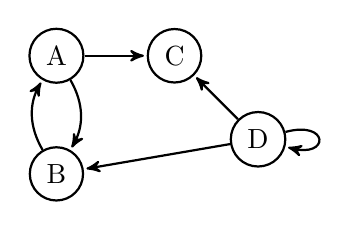
\begin{tikzpicture}[->,>=stealth',shorten >=1pt,auto,node distance=1.5cm,
 thick,main node/.style={circle,draw}]

  \node[main node] (A) [] {A};
  \node[main node] (B) [below of=A] {B};
  \node[main node] (C) [right of=A] {C};
  \node[main node] (D) [below right of=C] {D};

  \foreach \s/\t in {A/C, D/B, D/C} {
   \path[draw] (\s) edge (\t);}
    
  \path[]
 	(A) edge [bend left]  (B)
	(B) edge [bend left]  (A)
 	(D) edge [loop right] (D);

\end{tikzpicture}
\end{center}
\column{.5\textwidth}
\begin{itemize}
\item An example path:
\begin{itemize}
\item $D, B, A, C$
\end{itemize}
\item $D$ is the head.
\item $C$ is the tail.

\end{itemize}

\end{columns}
\end{frame}

%-----------------------------------------------
\begin{frame}
\frametitle{Definitions}
\begin{itemize}
\item A \textbf{cycle} is a path where the head and the tail are the same.
\item A graph without cycles is a \textbf{forest}.
\end{itemize}

\begin{columns}[c]
\column{.5\textwidth}

\begin{center}

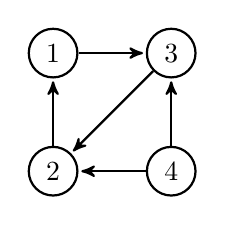
\begin{tikzpicture}[->,>=stealth',shorten >=1pt,auto,node distance=1.5cm,
 thick,main node/.style={circle,draw}]

  \node[main node] (1) [] {1};
  \node[main node] (2) [below of=1] {2};
  \node[main node] (3) [right of=1] {3};
  \node[main node] (4) [below of =3] {4};

  \foreach \s/\t in {1/3, 4/2, 4/3, 3/2, 2/1} {
   \path[draw] (\s) edge (\t);}
    
%  \path[]
 %	(A) edge [bend left]  (B)
%	(B) edge [bend left]  (A)
 %	(D) edge [loop right] (D);

\end{tikzpicture}

This graph contains cycles.

$2,1,3,2$ is a cycle.
\end{center}

\column{.5\textwidth}
\begin{center}


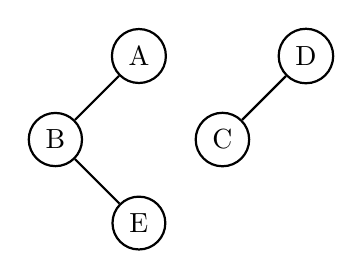
\begin{tikzpicture}[auto,node distance=1.5cm,
 thick,main node/.style={circle,draw}]
 
  \node[main node] (A) [] {A};
  \node[main node] (B) [below left of=A] {B};
  \node[main node] (C) [below right of=A] {C};
  \node[main node] (D) [above right of=C] {D};
  \node[main node] (E) [below left of=C] {E};  
  
  \foreach \s/\t/\i in {B/A/ , B/E/, C/D/ } {
   \path[draw] (\s) edge node {\i} (\t);}

\end{tikzpicture}


This graph does not have cycles and thus is a forest.
\end{center}.

\end{columns}



\end{frame}

%--------------------------------------------------
\begin{frame}
\frametitle{Definitions}
  \begin{itemize}
  \item A graph is  \textbf{connected} when a path exists connecting any two vertices.
  \item A connected forest is a \textbf{tree}.
  \item An undirected graph is a tree if and only if there is a unique path between any two vertices.
  \item Examples of trees:
  \end{itemize}

\begin{columns}[c]
  \column{.5\textwidth}
    \begin{center}

      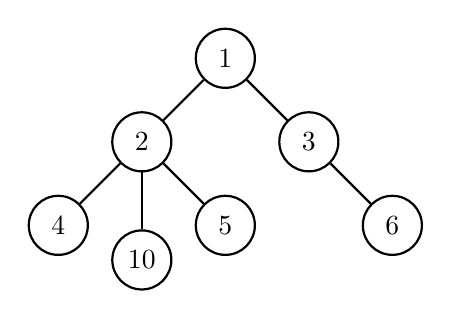
\begin{tikzpicture}[auto,node distance=1.5cm,
         thick,main node/.style={circle,draw}, minimum size=0.75cm] %Enlarged circle size to enable uniformity with double digit nodes
 
       \node[main node] (1) [] {1};
       \node[main node] (2) [below left of=1] {2};
       \node[main node] (3) [below right of=1] {3};
       \node[main node] (4) [below left of=2] {4};
       \node[main node] (5) [below right of=2] {5};
       \node[main node] (6) [below right of=3] {6};
       \node[main node] (10) [below of=2] {10};

       \foreach \s/\t in {2/1, 2/4, 2/5, 2/10, 3/1, 3/6} {
        \path[draw] (\s) edge (\t);}  
      \end{tikzpicture}

    \end{center}

  \column{.5\textwidth}
     \begin{center}

       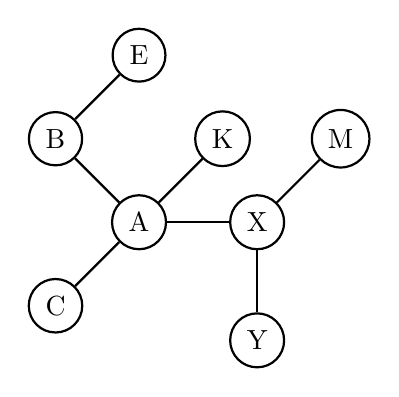
\begin{tikzpicture}[auto,node distance=1.5cm,
        thick,main node/.style={circle,draw}]
        \node[main node] (A) [] {A};
        \node[main node] (B) [above left of=A] {B};
        \node[main node] (C) [below left of=A] {C};
        \node[main node] (E) [above right of=B] {E};
        \node[main node] (K) [above right of=A] {K};
        \node[main node] (X) [right of=A] {X};
        \node[main node] (M) [above right of=X] {M};
        \node[main node] (Y) [below of=X] {Y};

        \foreach \s/\t in {A/B, A/C, A/K, A/X, B/E, X/M, X/Y} {
        \path[draw] (\s) edge (\t);}
        \end{tikzpicture}

    \end{center}

  \end{columns}

\end{frame}

%-------------------------------------------

\begin{frame}
\frametitle{Tree or Forest?}
\begin{columns}[c]

\column{.5\textwidth}
\begin{center}

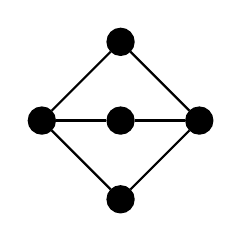
\begin{tikzpicture}[auto,node distance=1cm,
 thick,main node/.style={circle,draw, fill=black}]
  \node[main node] (1) [] {};
  \node[main node] (2) [above of=1] {};
  \node[main node] (3) [right of=1] {};
  \node[main node] (4) [left of=1] {};
  \node[main node] (5) [below of=1] {};

  \foreach \s/\t in {3/1, 3/2, 3/5, 4/1, 4/2, 4/5} {
   \path[draw] (\s) edge (\t);}
 \end{tikzpicture}
 
1. \only<2->{ Neither}


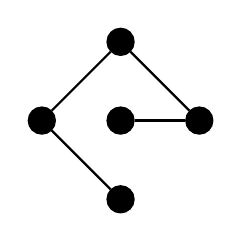
\begin{tikzpicture}[auto,node distance=1cm,
 thick,main node/.style={circle,draw, fill=black}]
  \node[main node] (1) [] {};
  \node[main node] (2) [above of=1] {};
  \node[main node] (3) [right of=1] {};
  \node[main node] (4) [left of=1] {};
  \node[main node] (5) [below of=1] {};

  \foreach \s/\t in {3/1, 3/2, 4/2, 4/5} {
   \path[draw] (\s) edge (\t);}  
 \end{tikzpicture}
 
2. \only<3->{Tree}

\end{center}

\column{.5\textwidth}
\begin{center}

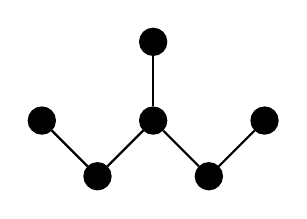
\begin{tikzpicture}[auto,node distance=1cm,
 thick,main node/.style={circle,draw, fill=black}]
  \node[main node] (1) [] {};
  \node[main node] (2) [below left of=1] {};
  \node[main node] (3) [below right of=1] {};
  \node[main node] (4) [above of=1] {};
  \node[main node] (5) [above left of=2] {};
  \node[main node] (6) [above right of=3] {};

  \foreach \s/\t in {1/2, 1/3, 1/4, 5/2, 6/3} {
   \path[draw] (\s) edge (\t);}  
 \end{tikzpicture}
 
3. \only<4->{Tree}

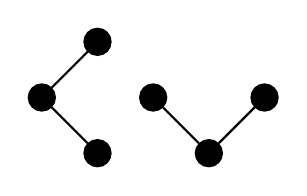
\begin{tikzpicture}[auto,node distance=1cm,
 thick,main node/.style={circle,draw, fill=black}]
  \node[main node] (1) [] {};
  \node[main node] (2) [below left of=1] {};
  \node[main node] (3) [below right of=1] {};
  \node[main node] (4) [above left of=2] {};
  \node[main node] (5) [above right of=4] {};
  \node[main node] (6) [above right of=3] {};

  \foreach \s/\t in {3/1, 3/6, 4/2, 4/5} {
   \path[draw] (\s) edge (\t);}  
 \end{tikzpicture}
 
4. \only<5->{Forest}

\end{center}

\end{columns}
\end{frame}

%---------------------------------------------
\begin{frame}
\frametitle{Storing a Graph}
\begin{itemize}
\item There are two ways to store a graph in a data structure.
\item An \textbf{adjacency matrix}, $A = [a_{ij}]$,  is an $n$ x $n$ matrix, where $n$ is the number of nodes and where $a_{ij} =
	\begin{cases} 1 & \text{if $(v_i,v_j) \in E$}\\
	0 & \text{otherwise} \end{cases}$
\item An \textbf{adjacency list} is a list of lists, where the $i$th list has all the nodes the $i$th node is connected to. Often stored as a dictionary.
\end{itemize}
\end{frame}

%---------------------------------------------

\begin{frame}
\frametitle{Storing a Graph Example}
\begin{columns}[c]
\column{.5\textwidth}
\begin{center}
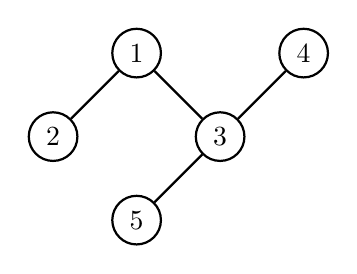
\begin{tikzpicture}[auto,node distance=1.5cm,
 thick,main node/.style={circle,draw}]
 
  \node[main node] (1) [] {1};
  \node[main node] (2) [below left of=1] {2};
  \node[main node] (3) [below right of=1] {3};
  \node[main node] (4) [above right of=3] {4};
  \node[main node] (5) [below left of=3] {5};  
  
  \foreach \s/\t/\i in {2/1/ , 3/1/, 3/4/, 3/5/ } {
   \path[draw] (\s) edge node {\i} (\t);}

\end{tikzpicture}
\end{center}

\column{.5\textwidth}
Adjacency matrix:
\[
\begin{pmatrix}
0 & 1 & 1 & 0 & 0 \\
1 & 0 & 0 & 0 & 0 \\
1 & 0 & 0 & 1 & 1 \\
0 & 0 & 1 & 0 & 0 \\
0 & 0 & 1 & 0 & 0 
\end{pmatrix}
\]

Adjacency list:
\[
\begin{tabular}{| l | l |}
\hline
1 & 2,3 \\
2 & 1 \\
3 & 1,4,5 \\
4 & 3 \\
5 & 3 \\
\hline
\end{tabular}
\]
\end{columns}
\end{frame}

%-------------------------------------------

\begin{frame}
\frametitle{Sparse and Dense}

\begin{itemize}
\item An adjacency matrix takes $|V|^2$ memory while an adjacency list takes $2|E| + |V|$.
\item If a graph is connected then $|V| \leq |E| \leq |V|^2$.
\item A graph is \textbf{sparse} if $|E|$ is close to $|V|$.
\item A graph is \textbf{dense} if $|E|$ is close to $|V|^2$.
\end{itemize}
\end{frame}

%-------------------------------------------
\begin{frame}
\frametitle{Directed Acyclic Graphs}
\begin{itemize}
\item A \textbf{directed acyclic graph} (DAG) or \textbf{acyclic digraph} is a simple directed graph with no cycles.
\item Every DAG has at least one \textbf{source} and one \textbf{sink}.
\end{itemize}

\begin{columns}[c]

\column{.6\textwidth}
\begin{center}

  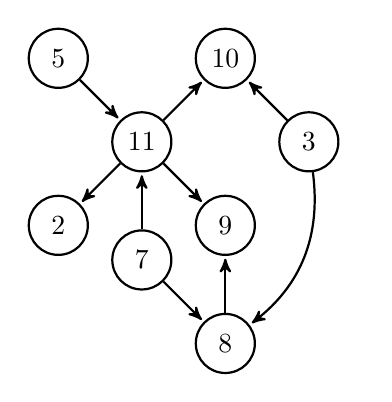
\begin{tikzpicture}[->,>=stealth',shorten >=1pt,auto,node distance=1.5cm,
 thick,main node/.style={circle,draw}, minimum size=.75cm]
   \node[main node] (9) [] {9};
   \node[main node] (3) [above right of=9] {3};
   \node[main node] (11) [above left of=9] {11};
   \node[main node] (8) [below of=9] {8};
   \node[main node] (10) [above left of=3] {10};
   \node[main node] (5) [above left of=11] {5};
   \node[main node] (7) [below of=11] {7};
   \node[main node] (2) [below left of=11] {2};

  \foreach \s/\t in {3/10, 5/11, 7/8, 7/11, 8/9, 11/2, 11/9, 11/10} {
   \path[draw] (\s) edge (\t);}   
  \path[]
	(3) edge [bend left] node {} (8);   
  \end{tikzpicture}

\end{center}

\column{.4\textwidth}
\begin{itemize}
\item $3,5$, and $7,$ are sources.

\item $2, 9,$ and $10$ are sinks.
\end{itemize}


\end{columns}

\end{frame}

%------------------------------------------

\begin{frame}
\frametitle{DAG Facts}

  \begin{itemize}
  \item Good for causalities, hierarchies, and temporal dependencies.
  \item Can be linearized, i.e. topologically sorted into a line.
  \item A generalization of trees.
  \end{itemize}

\begin{columns}[c]


    \column{.3\textwidth}
     \begin{center}
       
      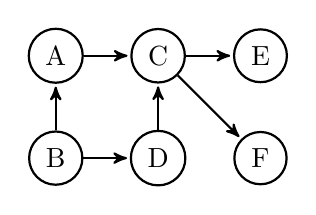
\begin{tikzpicture}[->,>=stealth',shorten >=1pt,auto,node distance=1.3cm,
      thick,main node/.style={circle,draw}]

      \node[main node] (A) [] {A};
      \node[main node] (B) [below of=A] {B};
      \node[main node] (C) [right of=A] {C};
      \node[main node] (D) [below of=C] {D};
      \node[main node] (E) [right of=C] {E};
      \node[main node] (F) [right of=D] {F};

      \foreach \s/\t in {A/C, B/A, B/D, C/E, C/F, D/C} {
          \path[draw] (\s) edge (\t);}
      \end{tikzpicture}
      
    A DAG
  \end{center}

\column{.7\textwidth}
  \begin{center}
  
  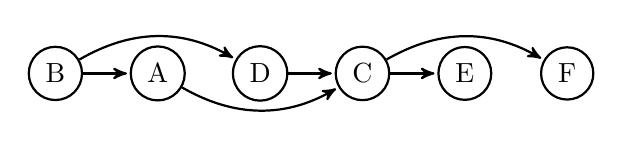
\begin{tikzpicture}[->,>=stealth',shorten >=1pt,auto,node distance=1.3cm,
 thick,main node/.style={circle,draw}]
  \node[main node] (B) [] {B};
  \node[main node] (A) [right of=B] {A};
  \node[main node] (D) [right of=A] {D};
  \node[main node] (C) [right of=D] {C};
  \node[main node] (E) [right of=C] {E};
  \node[main node] (F) [right of=E] {F};

 \foreach \s/\t in {B/A, C/E, D/C} {
   \path[draw] (\s) edge (\t);}
  
 \path[]
	(A) edge[bend right] (C)
	(B) edge[bend left] (D)
	(C) edge[bend left] (F);
 \end{tikzpicture}
 
  The linearized DAG
  \end{center}

\end{columns}

\end{frame}

%---------------------------------------------
\begin{frame}
\frametitle{DAG Facts}

\begin{columns}[c]
\column{.5\textwidth}

\begin{itemize}
%\item $A$ is an adjacency matrix of a DAG, if and only if $I+A$ has all positive eignevalues. TODO: need a new place for this fact
\item A \textbf{strongly connected component} is a subgraph where if there is a path from $x$ to $y$ then there is a path from $y$ to $x$.
%TODO: Check def doesn't match the example.
\item Every directed graph is a DAG of its strongly connected components.
\item The yellow circles show the strongly connected components.
\end{itemize}

\column{.5\textwidth}
\begin{center}

  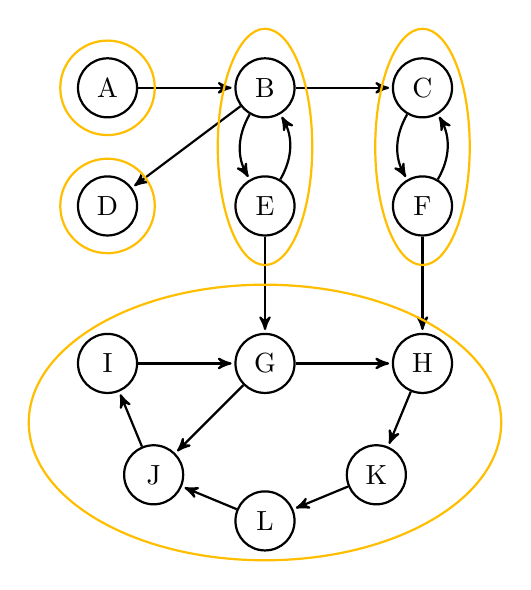
\begin{tikzpicture}[->,>=stealth',shorten >=1pt,auto,node distance=1.5cm,
 thick,main node/.style={circle,draw}, minimum size=.75cm]
  \node[main node] (A) [] {A};
  \node[main node] (D) [below of=A] {D};
  \node[main node, node distance = 2cm] (B) [right of=A] {B};
  \node[main node, node distance = 2cm] (C) [right of=B] {C};
  \node[main node] (E) [below of=B] {E};
  \node[main node, node distance = 2cm] (G) [below of=E] {G};
  \node[main node, node distance = 2cm] (J) [below left of=G] {J};
  \node[main node, node distance = 2cm] (I) [below of=D] {I};
  \node[main node] (F) [below of=C] {F};
  \node[main node, node distance = 2cm] (H) [below of=F] {H};
  \node[main node, node distance=2cm] (L) [below of=G] {L};
  \node[main node, node distance=2cm] (K) [below right of=G] {K};
 
  \foreach \s/\t in {A/B, B/C, B/D, E/G, F/H, G/J, H/K, I/G, J/I, L/J, K/L, G/H} {
   \path[draw] (\s) edge (\t);}
  \foreach \s/\t in {B/E, C/F, E/B, F/C} {
   \path[draw] (\s) edge[bend right] (\t);}


 \draw[orange!50!yellow] (0, 0) circle [radius=.6cm];
 \draw[orange!50!yellow] (0, -1.5) circle [radius=.6cm];
 \draw[orange!50!yellow] (2, -.75) circle [x radius=.6cm, y radius=1.5cm];
 \draw[orange!50!yellow] (4, -.75) circle [x radius=.6cm, y radius=1.5cm];
 \draw[orange!50!yellow] (2, -4.25) circle [x radius=3cm, y radius=1.75cm];
 \end{tikzpicture} 


\end{center}
\end{columns}
\end{frame}


%-------------------------------------------------------------------------------------------
\begin{frame}
\frametitle{DAG Facts}

\begin{itemize}
\item  DAG of the graph from the previous slide.
\item Each vertex in the DAG represents a strongly connected component from before.
\end{itemize}

\begin{center}

  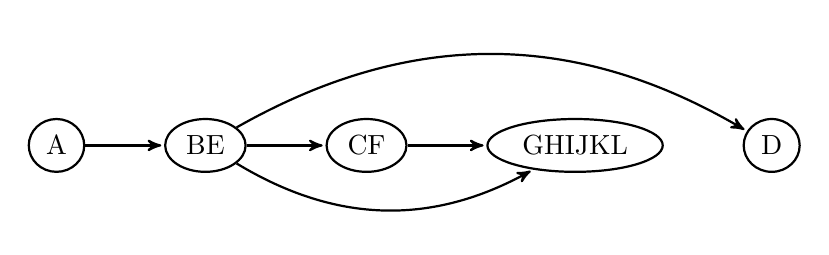
\begin{tikzpicture}[->,>=stealth',shorten >=1pt, auto,
 thick]
 \tikzstyle{block} = [ellipse, draw]
   \node[block] (A) [] {A};
   \node[block] (B) [right=1 cm of A] {BE}; %Used 1cm instead of 1.5cm because these ellipses are implemented as blocks.
   \node[block] (C) [right=1 cm of B] {CF};
   \node[block] (G) [right=1 cm of C] {GHIJKL};
   \node[block] (D) [right=1 cm of G] {D};
   
 \path[]
	(A) edge node {} (B)
	(B) edge node {} (C)
	     edge[bend right] node {} (G)
	     edge[bend left] node {} (D)
	(C) edge node {} (G);
  \end{tikzpicture}

\end{center}

\end{frame}

%----------------------------------------------
\begin{frame}
\frametitle{Classical DAG Problem}
\begin{itemize}
\item Find the longest increasing subsequence of the sequence $5, 2, 8, 6, 3, 6, 9, 7.$
\item This is solved by creating a DAG and then using backwards iteration.
\item Create the DAG by connecting each number to every greater number that comes after it in the sequence.
\end{itemize}

\begin{center}

  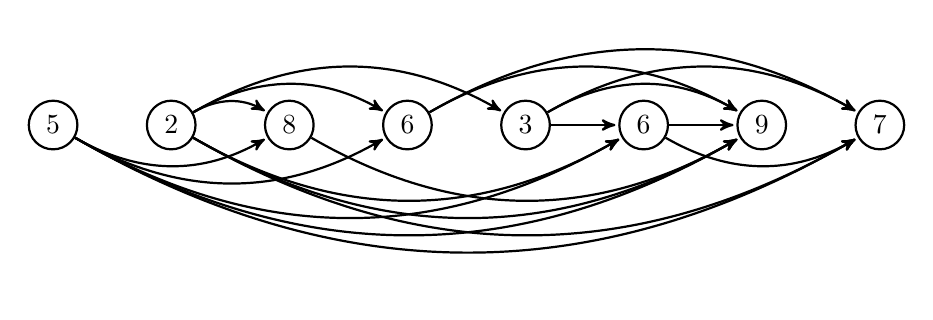
\begin{tikzpicture}[->,>=stealth',shorten >=1pt,auto,node distance=1.5cm,
 thick,main node/.style={circle,draw}]
 
  \node[main node] (5) [] {5};
  \node[main node] (2) [right of=5] {2};
  \node[main node] (8) [right of=2] {8};
  \node[main node] (6) [right of=8] {6};
  \node[main node] (3) [right of=6] {3};
  \node[main node] (2nd 6) [right of=3] {6};
  \node[main node] (9) [right of=2nd 6] {9};
  \node[main node] (7) [right of=9] {7};
  
  \foreach \s/\t in {5/8, 5/6, 5/2nd 6, 5/9, 5/7, 2/2nd 6, 2/7, 2/9, 8/9, 2nd 6/7} {
   \path[draw] (\s) edge[bend right] (\t);}

  \foreach \s/\t in {2/8, 2/6, 2/3, 6/9, 6/7, 3/9, 3/7} {
   \path[draw] (\s) edge[bend left] (\t);}
  
  \path[]
	(3) edge node {} (2nd 6)
	(2nd 6) edge node {} (9); 
 \end{tikzpicture}

\end{center}

\end{frame}
%----------------------------------------------
\begin{frame}
\frametitle{Classical DAG Problem}
\begin{itemize}
\item Iterate backwards by starting at the last node and tracing backwards through the DAG.
\item The longest increasing subsequence won't skip numbers.
\item Starting at 7, get $7, 6, 3, 2$. %TODO: it would be great to highlight the path in a different color!
\item Any other subsequences ending with 7 are shorter.
\end{itemize}
\begin{center}

  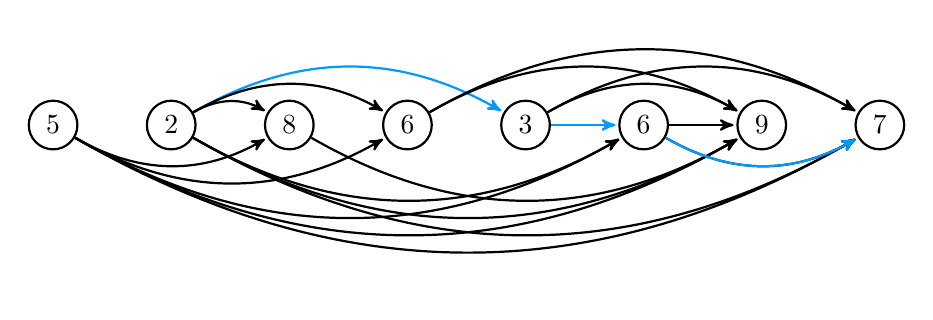
\begin{tikzpicture}[->,>=stealth',shorten >=1pt,auto,node distance=1.5cm,
 thick,main node/.style={circle,draw}]
 
  \node[main node] (5) [] {5};
  \node[main node] (2) [right of=5] {2};
  \node[main node] (8) [right of=2] {8};
  \node[main node] (6) [right of=8] {6};
  \node[main node] (3) [right of=6] {3};
  \node[main node] (2nd 6) [right of=3] {6};
  \node[main node] (9) [right of=2nd 6] {9};
  \node[main node] (7) [right of=9] {7};
  
  \foreach \s/\t in {5/8, 5/6, 5/2nd 6, 5/9, 5/7, 2/2nd 6, 2/7, 2/9, 8/9, 2nd 6/7} {
   \path[draw] (\s) edge[bend right] (\t);}
   
  \foreach \s/\t in {2nd 6/7} {
   \path[draw, blue!40!cyan] (\s) edge[bend right] (\t);}

  \foreach \s/\t in {2/3} {
   \path[draw, blue!40!cyan] (\s) edge[bend left] (\t);}

  \foreach \s/\t in {2/8, 2/6, 6/9, 6/7, 3/9, 3/7} {
   \path[draw] (\s) edge[bend left] (\t);}
  
  \path[blue!40!cyan]
	(3) edge node {} (2nd 6);
  \path[]
	(2nd 6) edge node {} (9); 
 \end{tikzpicture}

\end{center}
\end{frame}

%----------------------------------------------
\begin{frame}
\frametitle{Classical DAG Problem}
\begin{itemize}
\only<1>{\item Starting with 9, get $9, 6, 3, 2$.}
\only<2>{\item Next, $6, 3, 2$ is the longest ending in 6.
\item This has less than the other subsequences, so the algorithm ends.
\item $2, 3, 6, 7, $ and $2, 3, 6, 9$ are the longest increasing subsequences.}
\end{itemize}
\begin{center}

  \begin{tikzpicture}[->,>=stealth',shorten >=1pt,auto,node distance=1.5cm,
 thick,main node/.style={circle,draw}]
 
  \node[main node] (5) [] {5};
  \node[main node] (2) [right of=5] {2};
  \node[main node] (8) [right of=2] {8};
  \node[main node] (6) [right of=8] {6};
  \node[main node] (3) [right of=6] {3};
  \node[main node] (2nd 6) [right of=3] {6};
  \node[main node] (9) [right of=2nd 6] {9};
  \node[main node] (7) [right of=9] {7};
  
  \foreach \s/\t in {5/8, 5/6, 5/2nd 6, 5/9, 5/7, 2/2nd 6, 2/7, 2/9, 8/2nd 6, 2nd 6/7} {
   \path[draw] (\s) edge[bend right] (\t);}

  \foreach \s/\t in {2/8, 2/6, 6/9, 6/7, 3/9, 3/7} {
   \path[draw] (\s) edge[bend left] (\t);}
   
  \foreach \s/\t in {2/3} {
   \path[draw, blue!40!cyan] (\s) edge[bend left] (\t);}
  
  \path[blue!40!cyan]
	(3) edge node {} (2nd 6);
\only<1>{  \path[blue!40!cyan]
	(2nd 6) edge node {} (9); }
\only<2->{
 \path[]
	(2nd 6) edge node {} (9);
}
 \end{tikzpicture}

\end{center}
\end{frame}

%------------------------------------------------

\end{document}